\documentclass[a4paper,10pt]{article}
\usepackage[utf8]{inputenc}
\usepackage[T1]{fontenc}
\usepackage{kotex}
\usepackage{geometry}
\usepackage{amsmath,amssymb}
\usepackage{graphicx}
\usepackage{cite}
\usepackage{titlesec}
\usepackage{setspace}
\usepackage{xurl}

\geometry{
  left=18mm,
  right=18mm,
  top=22mm,
  bottom=20mm
}

\setstretch{1.08}
\setlength{\columnsep}{8mm}
\pagestyle{empty}
\emergencystretch=2em

\titleformat{\section}{\fontsize{11pt}{13pt}\selectfont\bfseries}{\thesection.}{0.5em}{}
\titleformat{\subsection}{\fontsize{10pt}{12pt}\selectfont\itshape}{\thesubsection}{0.5em}{}
\titlespacing*{\section}{0pt}{1.0ex plus 0.2ex minus 0.1ex}{0.5ex}
\titlespacing*{\subsection}{0pt}{0.8ex plus 0.2ex minus 0.1ex}{0.4ex}

\newcommand{\titlekr}[1]{{\fontsize{14pt}{16pt}\selectfont\bfseries #1\par}}
\newcommand{\titleen}[1]{{\fontsize{14pt}{16pt}\selectfont #1\par}}
\newcommand{\authorblock}[1]{{\fontsize{11pt}{13pt}\selectfont #1\par}}
\newcommand{\abstractfont}{\fontsize{11pt}{13pt}\selectfont}

\begin{document}
\twocolumn[
\begin{center}
\titlekr{악천후 조건 인식 기반 자율주행 위험 요소 탐지 및 추론 프레임워크}
\vspace{2mm}
\titleen{A Framework for Adverse Weather-Aware Hazard Detection and Reasoning in Autonomous Driving}
\vspace{4mm}
\authorblock{○양성렬$^{1}$, 지도교수$^{1*}$}
\vspace{2mm}
\authorblock{$^{1}$소속기관명 (TEL: 000-0000-0000, E-mail: kj458622@gmail.com)}
\end{center}

\vspace{4mm}
{\abstractfont
\noindent\textbf{Abstract}\enspace
Safety in autonomous driving requires not only object detection but also an understanding of why a scene is hazardous under current environmental conditions. Existing VLM-based hazard reasoning approaches focus on scene-level object identification but do not explicitly model how adverse weather conditions alter the nature and severity of risk. We propose a weather-aware hazard reasoning framework that injects a Structured Weather Context — comprising weather type, visibility, illumination, and road condition — alongside a front-view camera image into a pretrained VLM. Without task-specific fine-tuning, the framework produces structured outputs including hazard object, bounding box, risk level, and weather-causal explanation. Using Qwen2.5-VL-3B-Instruct on ACDC adverse-weather scenes, we qualitatively demonstrate that structured weather context injection shifts model outputs from scene-only description toward weather-grounded causal reasoning.\par}

\vspace{2mm}
{\abstractfont
\noindent\textbf{Keywords}\enspace
Autonomous Driving, Vision-Language Model, Hazard Reasoning, Adverse Weather, Structured Context Injection\par}
\vspace{4mm}
]

%% ────────────────────────────────────────────────
\section{서론}

자율주행 시스템의 안전성은 주변 객체를 인식하는 수준을 넘어, 현재 장면이 왜 위험한지 이해하고 설명할 수 있는 능력과 밀접하게 연결된다. 최근 Vision-Language Model(VLM)은 이미지와 언어를 함께 처리하며 장면 이해와 설명 생성에서 높은 성능을 보이고 있어 자율주행 hazard reasoning에 활발히 활용되고 있다~\cite{qwen2025}.

자율주행 분야에서는 안전 위협 요소를 탐지하고 설명하는 다양한 연구가 진행되어 왔다. INSIGHT~\cite{insight2026}는 Qwen2-VL을 기반으로 위험 영역의 위치와 위험 이유를 함께 설명하는 방향을 제시하였으며, 멀티태스크 학습을 통해 spatial grounding과 텍스트 설명을 동시에 생성한다. SADWA~\cite{sadwa2025}는 VLM에 날씨 인식 능력을 부여하려는 시도를 하였으나, hazard reasoning과의 직접적 연계는 다루지 않는다. 또한 ACDC~\cite{acdc2021}와 같은 악천후 데이터셋 연구는 열악한 환경에서의 perception 성능 저하 문제를 제기하였으나, 날씨가 위험 요소의 해석 자체를 어떻게 바꾸는지에 대한 설명은 충분하지 않다.

이러한 기존 연구들은 공통적으로 날씨·시정·노면 상태와 같은 환경 조건이 hazard 판단 자체를 어떻게 변화시키는지 구조적으로 반영하지 않는다. 실제 도로에서는 동일한 보행자·자전거 장면이라도 안개, 비, 눈 조건에 따라 위험의 성격과 대응 여유가 근본적으로 달라진다.

본 연구는 이러한 한계를 완화하기 위해, 단일 전방 카메라 이미지와 Structured Weather Context를 함께 VLM에 입력하는 weather-aware hazard reasoning 프레임워크를 제안한다. 본 프레임워크의 기여는 다음과 같다.

\begin{itemize}
  \setlength{\itemsep}{0pt}
  \item 악천후 조건을 구조화된 컨텍스트로 VLM에 주입하는 Structured Weather Context Injection 방식 제안
  \item Hazard object의 bounding box 탐지와 날씨 원인 기반 explanation을 동시에 생성하는 구조화된 출력 스키마 설계
  \item ACDC 데이터셋 기반 정성 실험을 통해 weather context가 hazard 탐지 및 위험 원인 설명을 실질적으로 변화시킴을 검증
\end{itemize}

%% ────────────────────────────────────────────────
\section{제안 방법}

\subsection{문제 정의}

본 연구는 단일 전방 이미지 $I$와 structured weather context $w$를 함께 사용하여 hazard reasoning 출력 $y$를 생성하는 문제를 다룬다.
%
\begin{equation}
  y = f_{\theta}(I,\, w)
\end{equation}
%
weather context는 네 필드로 구성된다.
%
\begin{equation}
  w = \{w_{\text{type}},\ v,\ l,\ r\}
\end{equation}
%
여기서 $w_{\text{type}}$, $v$, $l$, $r$은 각각 weather type, visibility, illumination, road condition이다. 출력은 다음과 같이 정의한다.
%
\begin{equation}
  y = \{o,\ b,\ s,\ e\}
\end{equation}
%
여기서 $o$, $b$, $s$, $e$는 각각 hazard object, bounding box, risk level, weather-causal explanation이다.

\subsection{Structured Weather Context Injection}

제안 프레임워크의 핵심은 weather context를 구조화된 텍스트로 VLM 프롬프트에 주입하는 것이다. 이미지만으로도 VLM은 장면 내 객체를 인식할 수 있으나, 날씨 조건이 해당 객체의 위험도를 어떻게 가중시키는지에 대한 인과적 설명은 weather context 없이는 생성되지 않는다. 프롬프트는 날씨 조건 prefix와 구조화된 출력 포맷 지시로 구성되며, 모델이 hazard object 식별, bounding box 예측, 날씨 원인 기반 explanation을 순차적으로 생성하도록 유도한다.

\subsection{구현}

베이스 모델로 Qwen2.5-VL-3B-Instruct~\cite{qwen2025}를 사용하며, 4-bit quantization을 적용하여 제한된 GPU 환경(T4 15GB)에서 추론을 수행한다. Task-specific fine-tuning은 수행하지 않으며, structured prompt conditioning만으로 weather-aware reasoning을 유도한다. 데이터셋은 ACDC~\cite{acdc2021} adverse-weather 이미지 중 snow, rain, fog 조건의 14장을 사용하였다.

그림~\ref{fig:pipeline}에 전체 파이프라인을 나타낸다.

\begin{figure}[h]
  \centering
  % 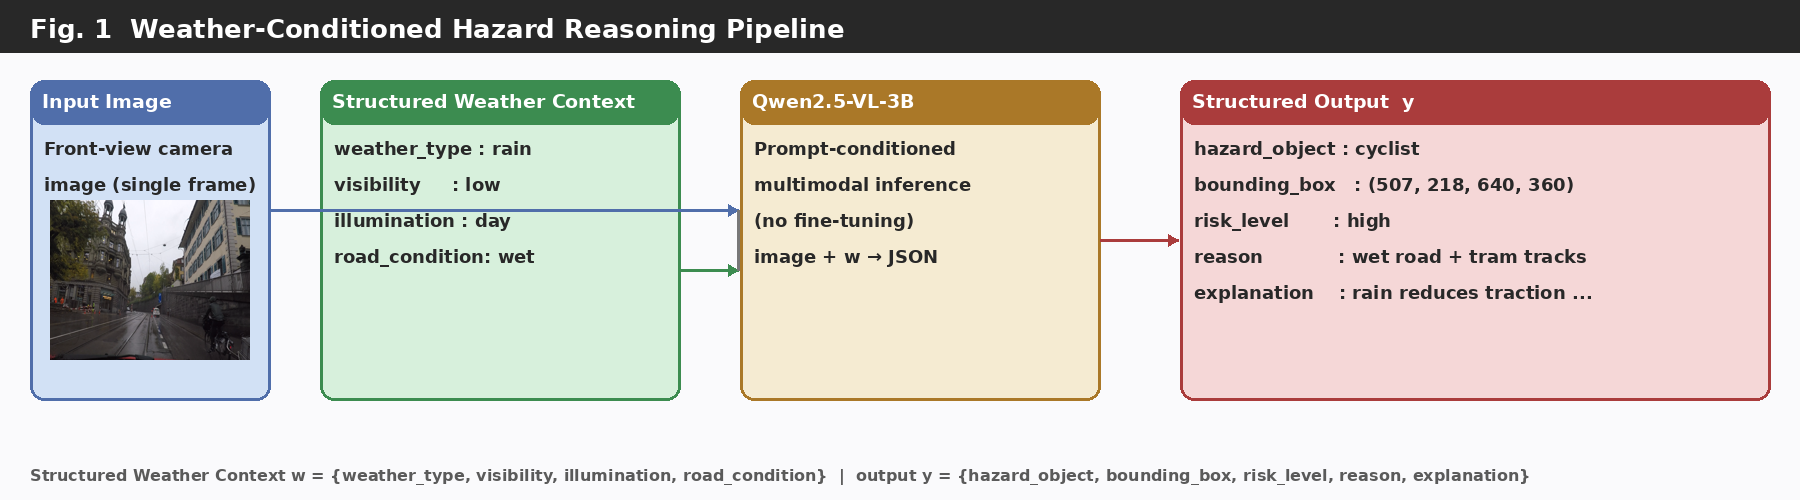
\includegraphics[width=\columnwidth]{figure_pipeline.png}
  \fbox{\rule{0pt}{2.5cm}\rule{\columnwidth}{0pt}}
  \caption{제안 프레임워크의 파이프라인. 전방 카메라 이미지와 Structured Weather Context를 Qwen2.5-VL-3B에 입력하여 hazard object, bounding box, risk level, weather-causal explanation을 출력한다.}
  \label{fig:pipeline}
\end{figure}

%% ────────────────────────────────────────────────
\section{실험 결과}

\subsection{정성적 결과}

그림~\ref{fig:qualitative}은 snow, rain, fog 조건에서의 대표적인 hazard reasoning 결과를 보여준다. 각 결과는 위험 객체의 bounding box와 함께 날씨 조건이 위험도를 어떻게 가중시키는지에 대한 설명을 포함한다.

\begin{figure}[h]
  \centering
  % 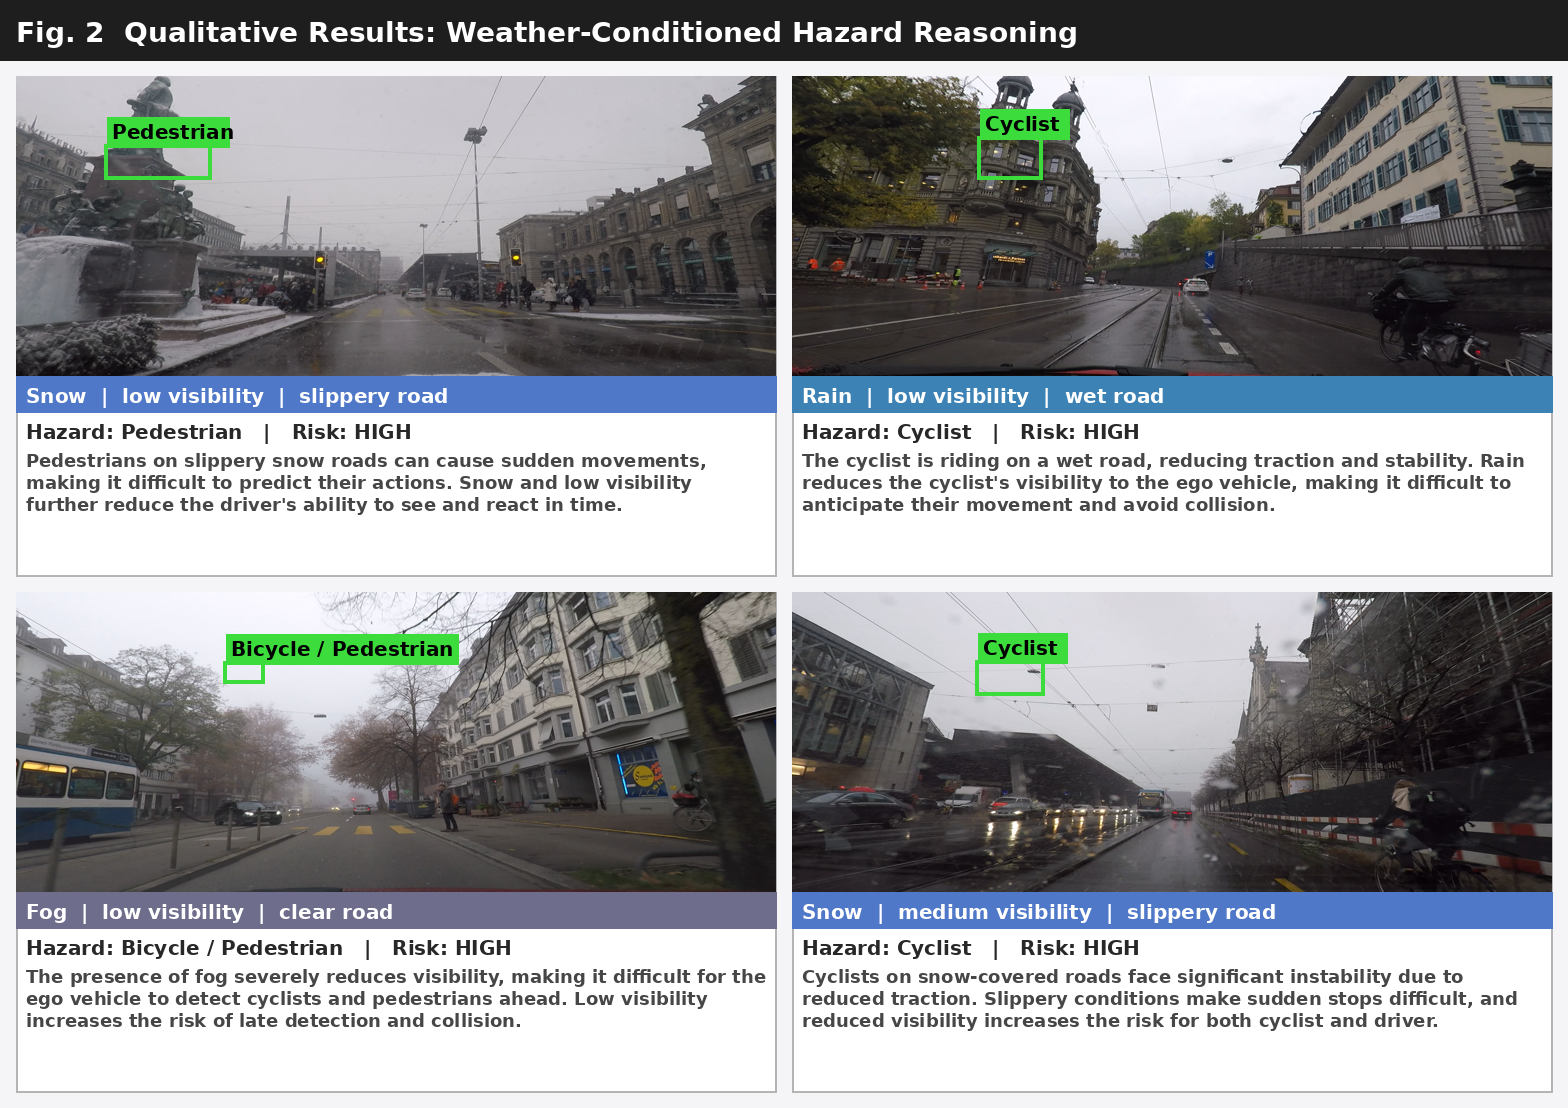
\includegraphics[width=\columnwidth]{figure_qualitative.png}
  \fbox{\rule{0pt}{5.0cm}\rule{\columnwidth}{0pt}}
  \caption{악천후 조건별 Hazard Reasoning 정성적 결과. (좌상) Snow: 보행자, 눈길 미끄러움으로 인한 반응 지연. (우상) Rain: 자전거, 빗길 마찰 감소 및 가시성 저하. (좌하) Fog: 자전거/보행자, 안개로 인한 객체 식별 어려움. (우하) Snow: 자전거, 눈 덮인 노면의 불안정성.}
  \label{fig:qualitative}
\end{figure}

\subsection{분석}

Weather context를 주입하지 않으면 모델은 장면 내 객체의 위치와 일반적 위험성만을 설명한다. 반면 weather context를 주입하면, 동일 장면에서 ``빗길로 인한 제동거리 증가'', ``안개로 인한 가시성 저하'', ``눈길의 미끄러움으로 인한 예측 불가능한 움직임'' 등 날씨가 위험을 가중시키는 인과적 설명이 생성된다. 이는 기존 scene-only reasoning이 제공하지 못하는 weather-conditioned causal explanation의 가능성을 보여준다.

%% ────────────────────────────────────────────────
\section{결론}

본 연구는 악천후 조건이 자율주행 hazard reasoning에 미치는 영향을 분석하고, Structured Weather Context Injection 기반의 weather-aware hazard reasoning 프레임워크를 제안하였다. Fine-tuning 없이 pretrained VLM에 구조화된 날씨 컨텍스트를 주입함으로써, 위험 객체의 bounding box 탐지와 함께 날씨 원인 기반의 hazard explanation 생성이 가능함을 정성적으로 검증하였다. 향후 연구로는 이미지 기반 자동 weather estimation, LoRA fine-tuning을 통한 출력 안정성 향상, INSIGHT의 spatial grounding과의 통합을 통해 보다 완성도 높은 시스템으로 발전시키고자 한다.

%% ────────────────────────────────────────────────
\begin{thebibliography}{9}

\bibitem{qwen2025}
Qwen Team, ``Qwen2.5-VL Technical Report,'' 2025.

\bibitem{insight2026}
D. Chen, Z. Zhang, L. Cheng, Y. Liu, and X. T. Yang,
``INSIGHT: Enhancing Autonomous Driving Safety through Vision-Language Models on Context-Aware Hazard Detection and Reasoning,''
\textit{arXiv}:2502.00262, 2026.

\bibitem{acdc2021}
C. Sakaridis, D. Dai, and L. Van Gool,
``ACDC: The Adverse Conditions Dataset with Correspondences for Semantic Driving Scene Understanding,''
\textit{Proc. ICCV}, 2021.

\bibitem{sadwa2025}
J. Kim et al.,
``SADWA: Fine-Grained Weather Awareness with Vision-Language Models for Seamless Autonomous Driving,''
\textit{ICCVW}, 2025.

\end{thebibliography}

\end{document}
